\documentclass[../../FisicaTeorica.tex]{subfiles}

\begin{document}

\section{Lezione ?:\\ \large{Titolo}}
\vspace{-1em}
\begin{center}
    \small{(15/11/2018)}
\end{center}

Scorsa lezione abbiamo visto che $A$ e $B$ sono osservabili compatibili se e solo se commutano.\\
$A$ e $B$ possono essere (banalmente) compatibili se uno è una funzione dell'altro, $B=f(A)$. Si dicono allora \textbf{dipendenti}, e le misure di una determinano le misure dell'altra.
In particolare si avrà $\sigma(B)=\sigma(f(A))=f(\sigma(A))$.\\
Altrimenti si dicono \textbf{indipendenti}.\\
Notiamo che la dipendenza di osservabili compatibili è soggetta a verifica sperimentale (possiamo misurare entrambe le osservabili e vedere se il valore di una coincide con $f$ calcolata nel valore dell'altra).\\
\begin{dfn}
Un insieme $\mathcal{C}$ di osservabili compatibili indipendenti si dice \textbf{completo} se è massimale, ossia se non esiste alcun insieme di osservabili compatibili indipendenti che lo contenga propriamente (non posso trovare insiemi \q{più grandi} strettamente). Quindi $\mathcal{C}$ è completo se una qualunque misura di I specie di un'ulteriore osservabile indipendente comporta necessariamente l'aumento delle fluttuazioni di almeno una delle osservabili di $\mathcal{C}$ (ossia eseguire una misura di un qualsiasi osservabile non compresa tra quelle in $\mathcal{C}$ \textit{disturba} quelle delle osservabili in $\mathcal{C}$).
\end{dfn}
Per le osservabili a spettro discreto, il risultato di una misura di I specie è l'individuazione del sottospazio di $\hs$ corrispondente all'autovalore trovato (quello \textit{compatibile} con la misura ottenuta).\\
Perciò la definizione di
\q{Completo} suggerisce la possibilità di ottenere informazione massimale sul sistema $\Rightarrow $ con la misura di un solo stato.\\

\begin{thm}
Sia $\mathcal{C}=\{A_1, \dots, A_n\}$ un insieme di osservabili compatibili indipendenti a spettro discreto. Allora $\mathcal{C}$ è completo se e solo se le osservabili $A_1, \dots, A_n$ hanno un insieme completo (cioè una base tale da verificare la completezza di Dirac) di autovettori comuni \textbf{nondegenere}.
\end{thm} 
\textbf{Dim}. Partiamo dimostrando che \textit{non degenere} $\Rightarrow$ \textit{completo}.         
Sia $B$ un'osservabile compatibile con $\mathcal{C}$ e sia $\{(\ket{(a_1,\dots, a_n)}\}$ con $(a_1, \dots, a_n)$ che denota gli autovalori comuni di $A_1, \dots, A_n$ ($\sigma(\mathcal{C})\neq \sigma(A_1)\times \dots \times \sigma(A_n)$).\\
Allora: (1)
\[
\sum_{(a_1 \dots a_n)\in \sigma(\mathcal{C})}= \ket{(a_1, \dots, a_n)}\bra{(a_1, \dots, a_n)}=\bb{I}
\]
(completezza di Dirac).\\
Poiché $B$ è compatibile con $\mathcal{C}$, ogni $\ket{(a_1, \dots, a_n)}$ deve essere autovettore di $B$ e quindi anche di $P^B(\lambda)$ la famiglia spettrale di $B$ per il teorema precedente (compatibilità con l'intera famiglia spettrale).\\
Quindi per qualche funzione $f_\lambda(a_1\dots a_n)$ vale: (2)
\[
P^B(\lambda)\ket{(a_1, \dots, a_n)}=f_\lambda(a_1, \dots, a_n) \ket{(a_1, \dots, a_n)}
\]
in modo univoco per la non-degenerazione.\\
Allora combinando (1) con (2) si ha:
\[
P^B(\lambda)\bb{I} = P^B(\lambda)=\sum_{(a_1, \dots, a_n)\in \sigma(\mathcal{C})} f_\lambda(a_1, \dots, a_n)\ket{(a_1, \dots, a_n)}\bra{(a_1, \dots, a_n)}\equiv f_\lambda(A_1,\dots, A_n)
\]
(dato che è la sua rappresentazione spettrale).\\
Quindi $B$ è una funzione di $\mathcal{C}$ individuata da:
\[
B=\int \lambda\,df_\lambda(A_1,\dots, A_n)
\]
ed è pertanto dipendente da $\mathcal{C}$, quindi $\mathcal{C}$ è completo.\\
Viceversa, dimostriamo che se vi è degenerazione $>1$ allora non si ha la completezza.\\
Se l'insieme di autovettori comuni di $\mathcal{C}$ ha degenerazione $\neq 1$, allora $\mathcal{C}$ non è completo.\\
Supponiamo che per qualche autovalore $(a_1, \dots, a_n) \in \sigma(\mathcal{C})$ l'autospazio $\hs_{(a_1,\dots,a_n)}$ abbia dimensione $d(a_1, \dots, a_n)>1$ (ossia vi è degenerazione).\\
Allora dato un operatore $B$ autoaggiunto non banale in $\hs_{(a_1,\dots, a_n)}$ (una qualsiasi matrice hermitiana in questo autospazio), esteso all'identità sul complemento di $\hs_{(a_1,\dots, a_n)}$ in $\hs$ (cioè lo estendo ad un operatore definito su tutto $\hs$ che è pari a $B$ sull'autospazio $\hs_{(a_1, \dots, a_n)}$, e agisce come l'identità su tutto il resto). Allora $B$ avrà la forma di \textit{matrice a blocchi}:
\[
B=
\begin{pmatrix}
\ddots & & &\\
& \bb{I} & &\\
& & B & &\\
& & & \bb{I} &\\
& & & & \ddots
\end{pmatrix}
\]
Questo operatore commuta con $A_1, \dots, A_n$, ma una misura di $A_1, \dots, A_n$ non determina il risultato di una misura di $B$.\\
Quindi $B$ è compatibile con $\mathcal{C}$ e indipendente, quindi $\mathcal{C}$ non è completo.
\begin{flushright}
$\square$
\end{flushright}

\begin{oss}
Poiché una misura su un Insieme Completo di Osservabili Compatibili (ICOC) $\mathcal{C}$ a spettro discreto identifica uno spazio $1-$dimensionale in $\hs$, tale misura può essere usata per preparare uno stato puro.
\end{oss}
\begin{oss}
Sotto opportune condizioni sugli spazi nucleari $\phi_{A_1,\dots,A_n}$ comuni a $\mathcal{C}$, il teorema precedente si estende ad un ICOC a spettro arbitrario, includendo gli autovettori generalizzati (cioè possiamo usarlo anche per \textit{spettri continui}).
\end{oss}
Questo consente di dare una definizione precisa di rappresentazione $\mathcal{C}$. Poiché per un ICOC $\mathcal{C}$ vale la completezza generalizzata, ossia:
\[
\prod_{i=1}^n \left(\sum_{a_i \in \sigma_P(A_i)} + \int_{\sigma_C(A_i)} da_i\right) \ket{(a_1,\dots,a_n)}\bra{(a_1,\dots,a_n)}=\bb{I}
\]
ove $\ket{(a_1, \dots, a_n)}$ sono autovettori (generalizzati) comuni di $\mathcal{C}$ \textbf{nondegeneri}, ogni vettore $\ket{(a_1, \dots, a_n)}$ è univocamente individuato dai valori $(a_1, \dots, a_n)$ e ogni $\ket{\psi}\in \hs$ si può scrivere:
\[
\ket{\psi}=\prod_{i=1}^n \left(\sum_{a_i\in \sigma_P(A_i)} + \int_{\sigma_C(A_i)}da_i \right) \ket{(a_1, \dots, a_n)}\braket{(a_1, \dots, a_n)|\psi}
\]
Quindi i coefficienti $\{\braket{(a_1, \dots, a_n)|\psi}=\psi(a_1, \dots, a_n)\}$, con $(a_1, \dots, a_n)\in \sigma(\mathcal{C})$, identificano univocamente lo stato $\ket{\psi}$ e vengono detti definire lo stato in \textbf{rappresentazione}$\mathcal{C}$.\\
Per esempio, supponiamo $\mathcal{C}=\{\vec{X}\}$, allora sappiamo che:
\[
\braket{\vec{x}|\psi}=\psi(\vec{x})
\]
Se invece $\mathcal{C}=\{\vec{P}\}$, allora:
\[
\braket{\vec{p}|\psi}=\tilde{\psi}(\vec{p})
\]
Per una particella in $\bb{R}^3$ potremmo scegliere $\mathcal{C}=\{X,P_y, Z\}$, on in $\bb{R}$ $\mathcal{C}=\{H, \mathcal{P}\}$, dato che se $[H,\mathcal{P}]=0$ \textit{rimuove} la degenerazione degli autovalori di $H$.

\begin{dfn}
Un insieme di osservabili $\mathcal{I}$ (non compatibili!) si dice \textbf{irriducibile} se ogni osservabile che commuta con tutti gli elementi di $\mathcal{I}$ è un multiplo dell'identità $\bb{I}$ (ossia il risultato della sua misura è indipendente dello stato - es. la carica elettrica dell'elettrone).\\
Possiamo ora caratterizzare una particella quantistica con un analogo \textit{classico}.
\end{dfn}

\begin{oss}
Per una particella quantistica elementare con analogo classico $\{\vec{x},\vec{p}\,\}$ è un insieme irriducibile.\\
Infatti sia $A$ un'osservabile che commuta con $\vec{X}$, poiché $\mathcal{C}=\{\vec{X}\}$ è un ICOC, necessariamente $A=f(\vec{X})$. Ma se $A$ commuta anche con $\vec{P}$, vuol dire che (usando la rappresentazione in $\vec{x}$):
\[
[\vec{P}, f(\vec{X})]\psi(\vec{X})=-i\hbar \vec{\nabla}(f(x)\psi(x))+i\hbar f(\vec{x})\vec{\nabla}\psi(\vec{x}) = -i\hbar(\vec{\nabla}f)(\vec{x})\psi(\vec{x})=0 \quad \forall \psi
\]
Ma allora:
\[
\vec{\nabla}f(\vec{x})=0=f(\vec{x})=\text{cost.}
\]
\end{oss}

\subsection{Esercizio}
Una particella di massa $m$ in 1D è immersa nel potenziale:
\[
V(x)=\begin{cases}
0 & |x|<\frac{a}{2}\\
+\infty & \text{altrove}
\end{cases}
\]
Sia $\mathcal{E}=\frac{2\pi^2\hbar^2}{ma^2}$ l'energia dello stato a $t=-t_0$ ($t_0>0$).
\begin{enumerate}
\item All'istante $t=0$ una misura (ideale di I specie) rivela la presenza della particella nella parte destra della buca. Determinare la funzione d'onda dopo la misura.
%[IMMAGINE] Disegnetto della buca con oscurata la parte sinistra (dove non è stata trovata la particella)
\item All'istante $t_0$ si esegue una misura\footnote{Che, quando non specificato diversamente, è da intendersi come ideale di prima specie}, determinare la probabilità di trovare un'energia più alta di quelle a $t=t_0$.
\item Determinare la probabilità di trovare il valore $+1$ eseguendo una misura di \textit{parità} $\mathcal{P}$ a $t=t_0$
\item Determinare $(\Delta X)_{\psi}(\Delta P)_\psi$ per tutti gli stati stazionari $\psi$\ del sistema.
\item Si dica se $P$ (con condizioni periodiche) e $H$ sono compatibili.
\item Si determini la probabilità di trovare la particella nella metà sinistra della buca per $0<t<t_0$.
\item Sette è un bel numero (ma per fortuna non c'è)
\end{enumerate}

\subsection{Soluzione}
\begin{enumerate}
\item Dalla soluzione della buca infinita sappiamo già che gli autovalori di $H$ sono:
\[
\mathcal{E}_n = \frac{\hbar^2}{2m}\frac{n^2 \pi^2}{a^2}
\]
e le rispettive autofunzioni sono:
\[
\varphi_n(x)=\begin{cases}
\sqrt{\frac{2}{a}}\cos\left(\frac{n\pi x}{a}\right) & n \in \bb{N} \text{ dispari }\\
\sqrt{\frac{2}{a}}\sin\left(\frac{n\pi x}{a}\right) & n\in \bb{N} \text{ pari}
\end{cases}
\]
\begin{figure}[H]
\centering
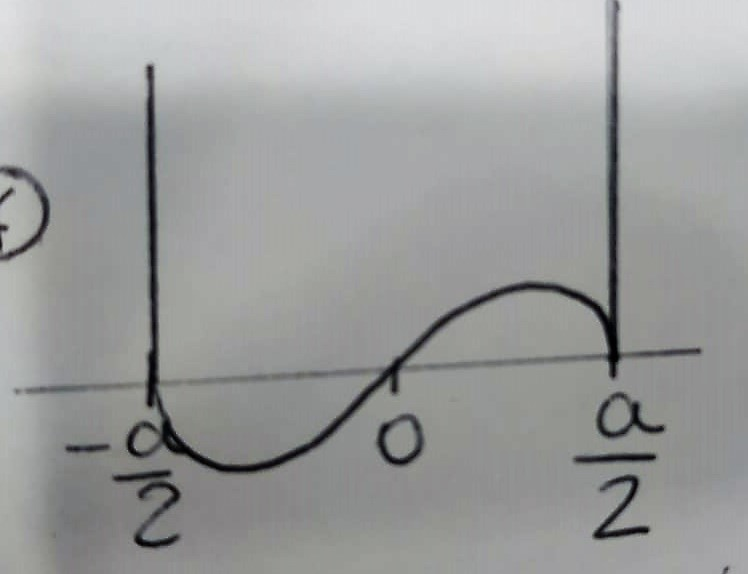
\includegraphics[scale=0.4]{Immagini/15_11/img2.jpeg}
\caption{$\psi$ iniziale}
\end{figure}
Notiamo che $\mathcal{E}=\mathcal{E}_2$ (chiaramente il valore assegnato \textbf{deve} essere uno di quelli possibili, al contrario di quanto accade in \MC).\\
Essendo lo stato a $t=-t_0$ autostato di $H$ rimane inalterato fino a che non si esegue una misura, cioè fino a $t=0$.\\
\begin{figure}[H]
\centering
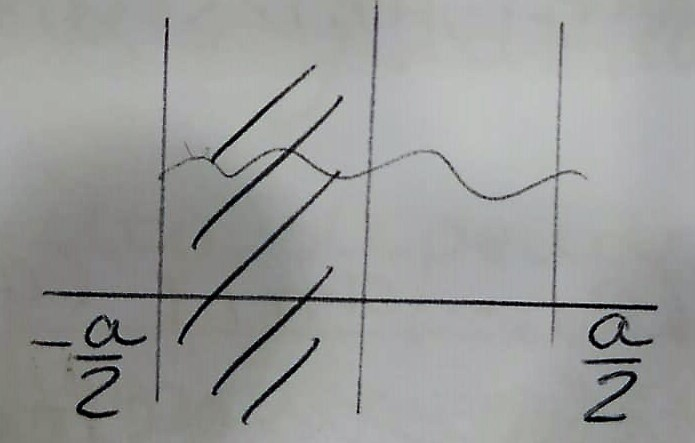
\includegraphics[scale=0.4]{Immagini/15_11/img1.jpeg}
\caption{Effetto della misura}
\end{figure}

\begin{figure}[H]
\centering
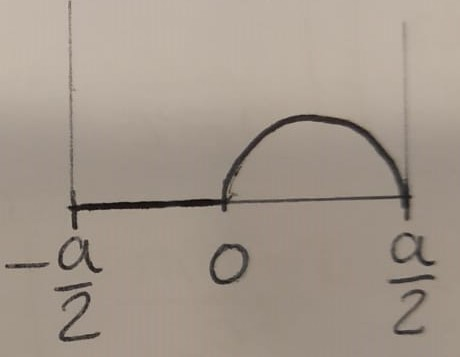
\includegraphics[scale=0.6]{Immagini/15_11/img3.jpeg}
\caption{$\psi$ dopo la misura}
\end{figure}
Matematicamente:
\[
\psi(x,t=0)=e^{-\frac{i}{\hbar}t_0\mathcal{E}_2} \psi(x,-t_0)
\]
Scegliendo opportunamente la fase, si ha che l'esponenziale non cambia nulla, e quindi:
\[
\psi(x,0^-)=\sqrt{\frac{2}{a}} \sin\left(\frac{2\pi x}{a}\right)
\]
Da cui la proiezione di von Neumann:
\[
\psi(x,0^+) = P^X\left(\left[0,\frac{a}{2}\right]\right)\psi(x,0^-)=A\begin{cases}
\sqrt{\frac{2}{a}}\sin\left(\frac{2\pi x}{a}\right) & 0 <x<\frac{a}{2}\\
0 & -\frac{a}{2}<x<0
\end{cases}
\]
Normalizziamo per trovare $A$:
\begin{align*}
1&\overset{!}{=}\int_{-\frac{a}{2}}^{+\frac{a}{2}} dx\,|\psi(x,0^+)|^2 = |A|^2 \int_0^{+\frac{a}{2}} \frac{2}{a}\sin^2\left(\frac{2\pi x}{a}\right)=\\
&=|A|^2 \int_0^{+\frac{a}{2}} \frac{2}{a}\frac{1}{2}\left(1-\cos\left(\frac{4\pi x}{a}\right)\right) dx = |A|^2 \frac{1}{a} \frac{a}{2} = \frac{|A|^2}{2}=1\Rightarrow A=\sqrt{2}
\end{align*}
Perciò:
\[
\psi(x,0^+)=\begin{cases}
\frac{2}{\sqrt{a}}\sin\left(\frac{2\pi x}{a}\right) & 0<x<+\frac{a}{2}\\
0 & -\frac{a}{2}<x<0
\end{cases}
\]
Per determinare $\psi(x,t)$ per $t>0$ (fino a $t_0$) dobbiamo espandere $\psi(x,0^+)$ negli autostati $\varphi_n(x)$ di $H$:
\[
\psi(x,0^+)=\sum_{n=1}^{\infty} \underbrace{(\varphi_n, \psi(0^+))}_{c_n}\varphi_n(x)
\]
Da cui:
\[
\psi(x,t)=\sum_{n=1}^\infty c_n e^{-\frac{i}{\hbar}\mathcal{E}_n t}\varphi_n(x)
\]
Per $n$ pari ($n$ dispari è lasciato come esercizio per casa):
\[
c_n = \int_{\bm{0}}^{+\frac{a}{2}} \sqrt{\frac{2}{a}} \sin\left(\frac{n\pi x}{a}\right) \frac{2}{\sqrt{a}}\sin\left(\frac{2\pi x}{a}\right)
\]
Applicando le formule di Werner:
\[
\sin(\alpha)\sin(\beta)=\frac{1}{2}(\cos(\alpha-\beta)-\cos(\alpha+\beta)
\]
Si ha che:
\[
c_n = \frac{2\sqrt{2}}{a}\int_0^{+\frac{a}{2}} \frac{1}{2}\cos \left[\cos \frac{(n-2)\pi x}{a}-\cos\frac{(n+2)\pi x}{a}\right]
\]
Per $n\neq 2$ si ottiene:
\[
\frac{\sqrt{2}}{a}\left[\frac{a}{(n-2)\pi}\sin\frac{(n-2)\pi x}{a}\right]\Big|_0^{+\frac{a}{2}} - \frac{a}{(n+2)\pi}\sin\frac{(n+2)\pi x}{a}\Big|_0^{+\frac{a}{2}}
\]
Per $n=2$ invece:
\[
\frac{\sqrt{2}}{a}\frac{a}{2}=\frac{1}{\sqrt{2}}
\]
\end{enumerate}
\end{document}

